\documentclass[twoside]{book}

% Packages required by doxygen
\usepackage{fixltx2e}
\usepackage{calc}
\usepackage{doxygen}
\usepackage[export]{adjustbox} % also loads graphicx
\usepackage{graphicx}
\usepackage[utf8]{inputenc}
\usepackage{makeidx}
\usepackage{multicol}
\usepackage{multirow}
\PassOptionsToPackage{warn}{textcomp}
\usepackage{textcomp}
\usepackage[nointegrals]{wasysym}
\usepackage[table]{xcolor}

% Font selection
\usepackage[T1]{fontenc}
\usepackage[scaled=.90]{helvet}
\usepackage{courier}
\usepackage{amssymb}
\usepackage{sectsty}
\renewcommand{\familydefault}{\sfdefault}
\allsectionsfont{%
  \fontseries{bc}\selectfont%
  \color{darkgray}%
}
\renewcommand{\DoxyLabelFont}{%
  \fontseries{bc}\selectfont%
  \color{darkgray}%
}
\newcommand{\+}{\discretionary{\mbox{\scriptsize$\hookleftarrow$}}{}{}}

% Page & text layout
\usepackage{geometry}
\geometry{%
  a4paper,%
  top=2.5cm,%
  bottom=2.5cm,%
  left=2.5cm,%
  right=2.5cm%
}
\tolerance=750
\hfuzz=15pt
\hbadness=750
\setlength{\emergencystretch}{15pt}
\setlength{\parindent}{0cm}
\setlength{\parskip}{3ex plus 2ex minus 2ex}
\makeatletter
\renewcommand{\paragraph}{%
  \@startsection{paragraph}{4}{0ex}{-1.0ex}{1.0ex}{%
    \normalfont\normalsize\bfseries\SS@parafont%
  }%
}
\renewcommand{\subparagraph}{%
  \@startsection{subparagraph}{5}{0ex}{-1.0ex}{1.0ex}{%
    \normalfont\normalsize\bfseries\SS@subparafont%
  }%
}
\makeatother

% Headers & footers
\usepackage{fancyhdr}
\pagestyle{fancyplain}
\fancyhead[LE]{\fancyplain{}{\bfseries\thepage}}
\fancyhead[CE]{\fancyplain{}{}}
\fancyhead[RE]{\fancyplain{}{\bfseries\leftmark}}
\fancyhead[LO]{\fancyplain{}{\bfseries\rightmark}}
\fancyhead[CO]{\fancyplain{}{}}
\fancyhead[RO]{\fancyplain{}{\bfseries\thepage}}
\fancyfoot[LE]{\fancyplain{}{}}
\fancyfoot[CE]{\fancyplain{}{}}
\fancyfoot[RE]{\fancyplain{}{\bfseries\scriptsize Generated by Doxygen }}
\fancyfoot[LO]{\fancyplain{}{\bfseries\scriptsize Generated by Doxygen }}
\fancyfoot[CO]{\fancyplain{}{}}
\fancyfoot[RO]{\fancyplain{}{}}
\renewcommand{\footrulewidth}{0.4pt}
\renewcommand{\chaptermark}[1]{%
  \markboth{#1}{}%
}
\renewcommand{\sectionmark}[1]{%
  \markright{\thesection\ #1}%
}

% Indices & bibliography
\usepackage{natbib}
\usepackage[titles]{tocloft}
\setcounter{tocdepth}{3}
\setcounter{secnumdepth}{5}
\makeindex

% Hyperlinks (required, but should be loaded last)
\usepackage{ifpdf}
\ifpdf
  \usepackage[pdftex,pagebackref=true]{hyperref}
\else
  \usepackage[ps2pdf,pagebackref=true]{hyperref}
\fi
\hypersetup{%
  colorlinks=true,%
  linkcolor=blue,%
  citecolor=blue,%
  unicode%
}

% Custom commands
\newcommand{\clearemptydoublepage}{%
  \newpage{\pagestyle{empty}\cleardoublepage}%
}

\usepackage{caption}
\captionsetup{labelsep=space,justification=centering,font={bf},singlelinecheck=off,skip=4pt,position=top}

%===== C O N T E N T S =====

\begin{document}

% Titlepage & ToC
\hypersetup{pageanchor=false,
             bookmarksnumbered=true,
             pdfencoding=unicode
            }
\pagenumbering{alph}
\begin{titlepage}
\vspace*{7cm}
\begin{center}%
{\Large My Project }\\
\vspace*{1cm}
{\large Generated by Doxygen 1.8.13}\\
\end{center}
\end{titlepage}
\clearemptydoublepage
\pagenumbering{roman}
\tableofcontents
\clearemptydoublepage
\pagenumbering{arabic}
\hypersetup{pageanchor=true}

%--- Begin generated contents ---
\chapter{Hierarchical Index}
\section{Class Hierarchy}
This inheritance list is sorted roughly, but not completely, alphabetically\+:\begin{DoxyCompactList}
\item \contentsline{section}{com.\+fware.\+cspdt.\+cspm.\+editor.\+config.\+Csp\+M\+Color\+Constants}{\pageref{enumcom_1_1fware_1_1cspdt_1_1cspm_1_1editor_1_1config_1_1_csp_m_color_constants}}{}
\item \contentsline{section}{com.\+fware.\+cspdt.\+cspm.\+editor.\+config.\+Csp\+M\+Color\+Manager}{\pageref{classcom_1_1fware_1_1cspdt_1_1cspm_1_1editor_1_1config_1_1_csp_m_color_manager}}{}
\item \contentsline{section}{com.\+fware.\+cspdt.\+cspm.\+editor.\+preferences.\+Csp\+M\+Editor\+Preference\+Constants}{\pageref{interfacecom_1_1fware_1_1cspdt_1_1cspm_1_1editor_1_1preferences_1_1_csp_m_editor_preference_constants}}{}
\item \contentsline{section}{com.\+fware.\+cspdt.\+cspm.\+editor.\+project.\+Csp\+M\+Project}{\pageref{classcom_1_1fware_1_1cspdt_1_1cspm_1_1editor_1_1project_1_1_csp_m_project}}{}
\item \contentsline{section}{com.\+fware.\+cspdt.\+cspm.\+editor.\+project.\+Csp\+M\+Project\+Properties}{\pageref{classcom_1_1fware_1_1cspdt_1_1cspm_1_1editor_1_1project_1_1_csp_m_project_properties}}{}
\item \contentsline{section}{com.\+fware.\+cspdt.\+cspm.\+editor.\+config.\+Keywords}{\pageref{enumcom_1_1fware_1_1cspdt_1_1cspm_1_1editor_1_1config_1_1_keywords}}{}
\item Abstract\+Preference\+Initializer\begin{DoxyCompactList}
\item \contentsline{section}{com.\+fware.\+cspdt.\+cspm.\+editor.\+preferences.\+Csp\+M\+Editor\+Preference\+Initializer}{\pageref{classcom_1_1fware_1_1cspdt_1_1cspm_1_1editor_1_1preferences_1_1_csp_m_editor_preference_initializer}}{}
\end{DoxyCompactList}
\item Abstract\+U\+I\+Plugin\begin{DoxyCompactList}
\item \contentsline{section}{com.\+fware.\+cspdt.\+cspm.\+editor.\+Csp\+M\+Editor\+Plugin}{\pageref{classcom_1_1fware_1_1cspdt_1_1cspm_1_1editor_1_1_csp_m_editor_plugin}}{}
\end{DoxyCompactList}
\item Content\+Outline\+Page\begin{DoxyCompactList}
\item \contentsline{section}{com.\+fware.\+cspdt.\+cspm.\+editor.\+outline.\+Csp\+M\+Content\+Outline\+Page}{\pageref{classcom_1_1fware_1_1cspdt_1_1cspm_1_1editor_1_1outline_1_1_csp_m_content_outline_page}}{}
\end{DoxyCompactList}
\item Csp\+Analyser\+Listener\begin{DoxyCompactList}
\item \contentsline{section}{com.\+fware.\+cspdt.\+cspm.\+editor.\+marker.\+Csp\+M\+Marking\+Error\+Handler}{\pageref{classcom_1_1fware_1_1cspdt_1_1cspm_1_1editor_1_1marker_1_1_csp_m_marking_error_handler}}{}
\end{DoxyCompactList}
\item Default\+Hyperlink\+Presenter\begin{DoxyCompactList}
\item \contentsline{section}{com.\+fware.\+cspdt.\+cspm.\+editor.\+link.\+Csp\+M\+Hyperlink\+Presenter}{\pageref{classcom_1_1fware_1_1cspdt_1_1cspm_1_1editor_1_1link_1_1_csp_m_hyperlink_presenter}}{}
\end{DoxyCompactList}
\item Default\+Indent\+Line\+Auto\+Edit\+Strategy\begin{DoxyCompactList}
\item \contentsline{section}{com.\+fware.\+cspdt.\+cspm.\+editor.\+config.\+Csp\+M\+Auto\+Indent\+Strategy}{\pageref{classcom_1_1fware_1_1cspdt_1_1cspm_1_1editor_1_1config_1_1_csp_m_auto_indent_strategy}}{}
\end{DoxyCompactList}
\item Extended\+Depth\+First\+Adapter\begin{DoxyCompactList}
\item \contentsline{section}{com.\+fware.\+cspdt.\+cspm.\+editor.\+link.\+Csp\+M\+Ref\+Extractor}{\pageref{classcom_1_1fware_1_1cspdt_1_1cspm_1_1editor_1_1link_1_1_csp_m_ref_extractor}}{}
\item \contentsline{section}{com.\+fware.\+cspdt.\+cspm.\+editor.\+outline.\+Csp\+M\+Ast\+Tree\+Node\+Generator}{\pageref{classcom_1_1fware_1_1cspdt_1_1cspm_1_1editor_1_1outline_1_1_csp_m_ast_tree_node_generator}}{}
\end{DoxyCompactList}
\item Fast\+Partitioner\begin{DoxyCompactList}
\item \contentsline{section}{com.\+fware.\+cspdt.\+cspm.\+editor.\+partition.\+Csp\+M\+Partitioner}{\pageref{classcom_1_1fware_1_1cspdt_1_1cspm_1_1editor_1_1partition_1_1_csp_m_partitioner}}{}
\end{DoxyCompactList}
\item Field\+Editor\+Preference\+Page\begin{DoxyCompactList}
\item \contentsline{section}{com.\+fware.\+cspdt.\+cspm.\+editor.\+preferences.\+Csp\+M\+Editor\+Preference\+Page}{\pageref{classcom_1_1fware_1_1cspdt_1_1cspm_1_1editor_1_1preferences_1_1_csp_m_editor_preference_page}}{}
\end{DoxyCompactList}
\item File\+Document\+Provider\begin{DoxyCompactList}
\item \contentsline{section}{com.\+fware.\+cspdt.\+cspm.\+editor.\+Csp\+M\+Document\+Provider}{\pageref{classcom_1_1fware_1_1cspdt_1_1cspm_1_1editor_1_1_csp_m_document_provider}}{}
\end{DoxyCompactList}
\item I\+Content\+Assist\+Processor\begin{DoxyCompactList}
\item \contentsline{section}{com.\+fware.\+cspdt.\+cspm.\+editor.\+config.\+Csp\+M\+Process\+Completion\+Processor}{\pageref{classcom_1_1fware_1_1cspdt_1_1cspm_1_1editor_1_1config_1_1_csp_m_process_completion_processor}}{}
\end{DoxyCompactList}
\item I\+Editor\+Part\begin{DoxyCompactList}
\item \contentsline{section}{com.\+fware.\+cspdt.\+cspm.\+editor.\+Csp\+M\+Editor}{\pageref{classcom_1_1fware_1_1cspdt_1_1cspm_1_1editor_1_1_csp_m_editor}}{}
\end{DoxyCompactList}
\item I\+Executable\+Extension\begin{DoxyCompactList}
\item \contentsline{section}{com.\+fware.\+cspdt.\+cspm.\+editor.\+wizards.\+Csp\+M\+New\+Project\+Wizard}{\pageref{classcom_1_1fware_1_1cspdt_1_1cspm_1_1editor_1_1wizards_1_1_csp_m_new_project_wizard}}{}
\end{DoxyCompactList}
\item I\+Hyperlink\begin{DoxyCompactList}
\item \contentsline{section}{com.\+fware.\+cspdt.\+cspm.\+editor.\+link.\+Csp\+M\+Hyperlink}{\pageref{classcom_1_1fware_1_1cspdt_1_1cspm_1_1editor_1_1link_1_1_csp_m_hyperlink}}{}
\end{DoxyCompactList}
\item I\+Hyperlink\+Detector\begin{DoxyCompactList}
\item \contentsline{section}{com.\+fware.\+cspdt.\+cspm.\+editor.\+link.\+Csp\+M\+Hyperlink\+Detector}{\pageref{classcom_1_1fware_1_1cspdt_1_1cspm_1_1editor_1_1link_1_1_csp_m_hyperlink_detector}}{}
\end{DoxyCompactList}
\item I\+New\+Wizard\begin{DoxyCompactList}
\item \contentsline{section}{com.\+fware.\+cspdt.\+cspm.\+editor.\+wizards.\+Csp\+M\+New\+File\+Wizard}{\pageref{classcom_1_1fware_1_1cspdt_1_1cspm_1_1editor_1_1wizards_1_1_csp_m_new_file_wizard}}{}
\item \contentsline{section}{com.\+fware.\+cspdt.\+cspm.\+editor.\+wizards.\+Csp\+M\+New\+Project\+Wizard}{\pageref{classcom_1_1fware_1_1cspdt_1_1cspm_1_1editor_1_1wizards_1_1_csp_m_new_project_wizard}}{}
\end{DoxyCompactList}
\item I\+Predicate\+Rule\begin{DoxyCompactList}
\item \contentsline{section}{com.\+fware.\+cspdt.\+cspm.\+editor.\+partition.\+Process\+Rule}{\pageref{classcom_1_1fware_1_1cspdt_1_1cspm_1_1editor_1_1partition_1_1_process_rule}}{}
\end{DoxyCompactList}
\item I\+Presentation\+Damager\begin{DoxyCompactList}
\item \contentsline{section}{com.\+fware.\+cspdt.\+cspm.\+editor.\+config.\+Non\+Rule\+Based\+Damager\+Repairer}{\pageref{classcom_1_1fware_1_1cspdt_1_1cspm_1_1editor_1_1config_1_1_non_rule_based_damager_repairer}}{}
\end{DoxyCompactList}
\item I\+Presentation\+Repairer\begin{DoxyCompactList}
\item \contentsline{section}{com.\+fware.\+cspdt.\+cspm.\+editor.\+config.\+Non\+Rule\+Based\+Damager\+Repairer}{\pageref{classcom_1_1fware_1_1cspdt_1_1cspm_1_1editor_1_1config_1_1_non_rule_based_damager_repairer}}{}
\end{DoxyCompactList}
\item I\+Reconciling\+Strategy\begin{DoxyCompactList}
\item \contentsline{section}{com.\+fware.\+cspdt.\+cspm.\+editor.\+config.\+Csp\+M\+Reconciling\+Strategy}{\pageref{classcom_1_1fware_1_1cspdt_1_1cspm_1_1editor_1_1config_1_1_csp_m_reconciling_strategy}}{}
\end{DoxyCompactList}
\item I\+Runnable\+With\+Progress\begin{DoxyCompactList}
\item \contentsline{section}{com.\+fware.\+cspdt.\+cspm.\+editor.\+wizards.\+Csp\+M\+New\+Project\+Operation}{\pageref{classcom_1_1fware_1_1cspdt_1_1cspm_1_1editor_1_1wizards_1_1_csp_m_new_project_operation}}{}
\end{DoxyCompactList}
\item I\+Text\+Double\+Click\+Strategy\begin{DoxyCompactList}
\item \contentsline{section}{com.\+fware.\+cspdt.\+cspm.\+editor.\+config.\+Csp\+M\+Double\+Click\+Strategy}{\pageref{classcom_1_1fware_1_1cspdt_1_1cspm_1_1editor_1_1config_1_1_csp_m_double_click_strategy}}{}
\end{DoxyCompactList}
\item I\+Text\+Hover\begin{DoxyCompactList}
\item \contentsline{section}{com.\+fware.\+cspdt.\+cspm.\+editor.\+hover.\+Csp\+M\+Text\+Hover}{\pageref{classcom_1_1fware_1_1cspdt_1_1cspm_1_1editor_1_1hover_1_1_csp_m_text_hover}}{}
\end{DoxyCompactList}
\item I\+Whitespace\+Detector\begin{DoxyCompactList}
\item \contentsline{section}{com.\+fware.\+cspdt.\+cspm.\+editor.\+scanner.\+Csp\+Whitespace\+Detector}{\pageref{classcom_1_1fware_1_1cspdt_1_1cspm_1_1editor_1_1scanner_1_1_csp_whitespace_detector}}{}
\end{DoxyCompactList}
\item I\+Word\+Detector\begin{DoxyCompactList}
\item \contentsline{section}{com.\+fware.\+cspdt.\+cspm.\+editor.\+scanner.\+Csp\+M\+Keyword\+Detector}{\pageref{classcom_1_1fware_1_1cspdt_1_1cspm_1_1editor_1_1scanner_1_1_csp_m_keyword_detector}}{}
\item \contentsline{section}{com.\+fware.\+cspdt.\+cspm.\+editor.\+scanner.\+Csp\+M\+Name\+Detector}{\pageref{classcom_1_1fware_1_1cspdt_1_1cspm_1_1editor_1_1scanner_1_1_csp_m_name_detector}}{}
\end{DoxyCompactList}
\item I\+Workbench\+Preference\+Page\begin{DoxyCompactList}
\item \contentsline{section}{com.\+fware.\+cspdt.\+cspm.\+editor.\+preferences.\+Csp\+M\+Editor\+Preference\+Page}{\pageref{classcom_1_1fware_1_1cspdt_1_1cspm_1_1editor_1_1preferences_1_1_csp_m_editor_preference_page}}{}
\end{DoxyCompactList}
\item Rule\+Based\+Partition\+Scanner\begin{DoxyCompactList}
\item \contentsline{section}{com.\+fware.\+cspdt.\+cspm.\+editor.\+partition.\+Csp\+M\+Partition\+Scanner}{\pageref{classcom_1_1fware_1_1cspdt_1_1cspm_1_1editor_1_1partition_1_1_csp_m_partition_scanner}}{}
\end{DoxyCompactList}
\item Rule\+Based\+Scanner\begin{DoxyCompactList}
\item \contentsline{section}{com.\+fware.\+cspdt.\+cspm.\+editor.\+scanner.\+Csp\+M\+Scanner}{\pageref{classcom_1_1fware_1_1cspdt_1_1cspm_1_1editor_1_1scanner_1_1_csp_m_scanner}}{}
\end{DoxyCompactList}
\item Text\+Editor\begin{DoxyCompactList}
\item \contentsline{section}{com.\+fware.\+cspdt.\+cspm.\+editor.\+Csp\+M\+Editor}{\pageref{classcom_1_1fware_1_1cspdt_1_1cspm_1_1editor_1_1_csp_m_editor}}{}
\end{DoxyCompactList}
\item Text\+Editor\+Action\+Contributor\begin{DoxyCompactList}
\item \contentsline{section}{com.\+fware.\+cspdt.\+cspm.\+editor.\+Csp\+M\+File\+Editor\+Contributor}{\pageref{classcom_1_1fware_1_1cspdt_1_1cspm_1_1editor_1_1_csp_m_file_editor_contributor}}{}
\end{DoxyCompactList}
\item Text\+Source\+Viewer\+Configuration\begin{DoxyCompactList}
\item \contentsline{section}{com.\+fware.\+cspdt.\+cspm.\+editor.\+config.\+Csp\+M\+Source\+Viewer\+Configuration}{\pageref{classcom_1_1fware_1_1cspdt_1_1cspm_1_1editor_1_1config_1_1_csp_m_source_viewer_configuration}}{}
\end{DoxyCompactList}
\item Tree\+Node\begin{DoxyCompactList}
\item \contentsline{section}{com.\+fware.\+cspdt.\+cspm.\+editor.\+outline.\+Csp\+M\+Outline\+Tree\+Node}{\pageref{classcom_1_1fware_1_1cspdt_1_1cspm_1_1editor_1_1outline_1_1_csp_m_outline_tree_node}}{}
\end{DoxyCompactList}
\item Tree\+Node\+Content\+Provider\begin{DoxyCompactList}
\item \contentsline{section}{com.\+fware.\+cspdt.\+cspm.\+editor.\+outline.\+Csp\+M\+Outline\+Content\+Provider}{\pageref{classcom_1_1fware_1_1cspdt_1_1cspm_1_1editor_1_1outline_1_1_csp_m_outline_content_provider}}{}
\end{DoxyCompactList}
\item Wizard\begin{DoxyCompactList}
\item \contentsline{section}{com.\+fware.\+cspdt.\+cspm.\+editor.\+wizards.\+Csp\+M\+New\+File\+Wizard}{\pageref{classcom_1_1fware_1_1cspdt_1_1cspm_1_1editor_1_1wizards_1_1_csp_m_new_file_wizard}}{}
\item \contentsline{section}{com.\+fware.\+cspdt.\+cspm.\+editor.\+wizards.\+Csp\+M\+New\+Project\+Wizard}{\pageref{classcom_1_1fware_1_1cspdt_1_1cspm_1_1editor_1_1wizards_1_1_csp_m_new_project_wizard}}{}
\end{DoxyCompactList}
\item Wizard\+Page\begin{DoxyCompactList}
\item \contentsline{section}{com.\+fware.\+cspdt.\+cspm.\+editor.\+wizards.\+Csp\+M\+New\+File\+Wizard\+Page}{\pageref{classcom_1_1fware_1_1cspdt_1_1cspm_1_1editor_1_1wizards_1_1_csp_m_new_file_wizard_page}}{}
\end{DoxyCompactList}
\end{DoxyCompactList}

\chapter{Class Index}
\section{Class List}
Here are the classes, structs, unions and interfaces with brief descriptions\+:\begin{DoxyCompactList}
\item\contentsline{section}{\hyperlink{classcom_1_1fware_1_1cspdt_1_1cspm_1_1core_1_1parser_1_1_csp_m_analyser_exception}{com.\+fware.\+cspdt.\+cspm.\+core.\+parser.\+Csp\+M\+Analyser\+Exception} \\*Excecao disparada quando a analise lexica de um no na ast falha }{\pageref{classcom_1_1fware_1_1cspdt_1_1cspm_1_1core_1_1parser_1_1_csp_m_analyser_exception}}{}
\item\contentsline{section}{\hyperlink{classcom_1_1fware_1_1cspdt_1_1cspm_1_1core_1_1_csp_m_core_plugin}{com.\+fware.\+cspdt.\+cspm.\+core.\+Csp\+M\+Core\+Plugin} \\*Classe principal do plug-\/in }{\pageref{classcom_1_1fware_1_1cspdt_1_1cspm_1_1core_1_1_csp_m_core_plugin}}{}
\item\contentsline{section}{\hyperlink{classcom_1_1fware_1_1cspdt_1_1cspm_1_1core_1_1model_1_1_csp_m_model}{com.\+fware.\+cspdt.\+cspm.\+core.\+model.\+Csp\+M\+Model} \\*Essa classe contera os dados de analise do codigo }{\pageref{classcom_1_1fware_1_1cspdt_1_1cspm_1_1core_1_1model_1_1_csp_m_model}}{}
\item\contentsline{section}{\hyperlink{classcom_1_1fware_1_1cspdt_1_1cspm_1_1core_1_1parser_1_1_csp_m_parser}{com.\+fware.\+cspdt.\+cspm.\+core.\+parser.\+Csp\+M\+Parser} \\*Uma classe para usar a analise lexica e sintatica do codigo C\+SP }{\pageref{classcom_1_1fware_1_1cspdt_1_1cspm_1_1core_1_1parser_1_1_csp_m_parser}}{}
\item\contentsline{section}{\hyperlink{classcom_1_1fware_1_1cspdt_1_1cspm_1_1core_1_1parser_1_1_csp_m_parser_exception}{com.\+fware.\+cspdt.\+cspm.\+core.\+parser.\+Csp\+M\+Parser\+Exception} \\*Excecao disparada quando a analise sintatica de um no na ast falha }{\pageref{classcom_1_1fware_1_1cspdt_1_1cspm_1_1core_1_1parser_1_1_csp_m_parser_exception}}{}
\item\contentsline{section}{\hyperlink{classcom_1_1fware_1_1cspdt_1_1cspm_1_1core_1_1model_1_1_csp_m_ref}{com.\+fware.\+cspdt.\+cspm.\+core.\+model.\+Csp\+M\+Ref} \\*Essa classe representa uma referencia dentro do documento C\+SP }{\pageref{classcom_1_1fware_1_1cspdt_1_1cspm_1_1core_1_1model_1_1_csp_m_ref}}{}
\item\contentsline{section}{\hyperlink{classcom_1_1fware_1_1cspdt_1_1cspm_1_1core_1_1model_1_1_token_extractor}{com.\+fware.\+cspdt.\+cspm.\+core.\+model.\+Token\+Extractor} \\*Classe que extrai tokens da ast }{\pageref{classcom_1_1fware_1_1cspdt_1_1cspm_1_1core_1_1model_1_1_token_extractor}}{}
\end{DoxyCompactList}

\chapter{Class Documentation}
\hypertarget{classcom_1_1fware_1_1cspdt_1_1cspm_1_1_csp_m_plugin}{}\section{com.\+fware.\+cspdt.\+cspm.\+Csp\+M\+Plugin Class Reference}
\label{classcom_1_1fware_1_1cspdt_1_1cspm_1_1_csp_m_plugin}\index{com.\+fware.\+cspdt.\+cspm.\+Csp\+M\+Plugin@{com.\+fware.\+cspdt.\+cspm.\+Csp\+M\+Plugin}}


Classe principal do plug-\/in.  


Inheritance diagram for com.\+fware.\+cspdt.\+cspm.\+Csp\+M\+Plugin\+:\begin{figure}[H]
\begin{center}
\leavevmode
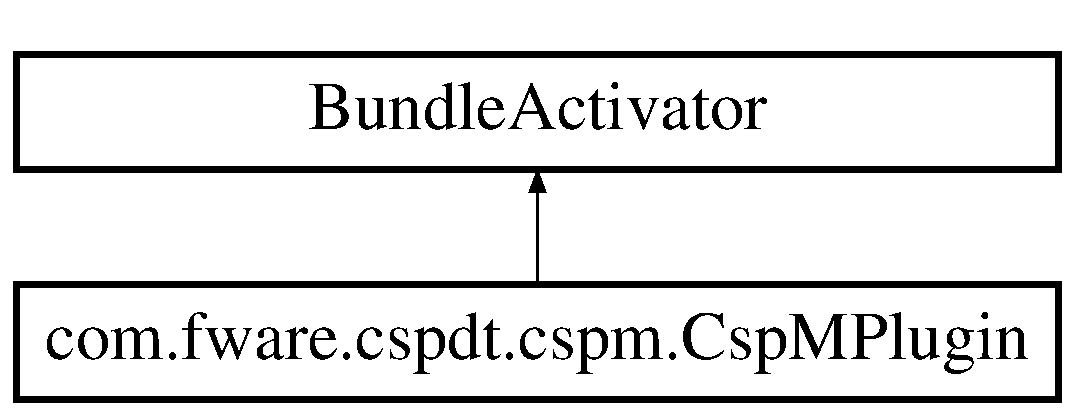
\includegraphics[height=2.000000cm]{classcom_1_1fware_1_1cspdt_1_1cspm_1_1_csp_m_plugin}
\end{center}
\end{figure}
\subsection*{Public Member Functions}
\begin{DoxyCompactItemize}
\item 
\mbox{\Hypertarget{classcom_1_1fware_1_1cspdt_1_1cspm_1_1_csp_m_plugin_accefd95fec71382913ef73d5fe6b90ff}\label{classcom_1_1fware_1_1cspdt_1_1cspm_1_1_csp_m_plugin_accefd95fec71382913ef73d5fe6b90ff}} 
void {\bfseries start} (Bundle\+Context bundle\+Context)  throws Exception 
\item 
\mbox{\Hypertarget{classcom_1_1fware_1_1cspdt_1_1cspm_1_1_csp_m_plugin_a38b9433569a3c47b29d7ef1911017346}\label{classcom_1_1fware_1_1cspdt_1_1cspm_1_1_csp_m_plugin_a38b9433569a3c47b29d7ef1911017346}} 
void {\bfseries stop} (Bundle\+Context bundle\+Context)  throws Exception 
\end{DoxyCompactItemize}


\subsection{Detailed Description}
Classe principal do plug-\/in. 

Contem o contexto que comunica com o Eclipse.

\begin{DoxyAuthor}{Author}
A\+L\+V\+A\+RO, E\+V\+E\+R\+A\+L\+DA, F\+E\+L\+I\+PE, J\+O\+N\+A\+T\+H\+AN, J\+U\+V\+E\+N\+AL 
\end{DoxyAuthor}


The documentation for this class was generated from the following file\+:\begin{DoxyCompactItemize}
\item 
C\+:/\+Users/\+E\+V\+A/\+Downloads/eclipse/workspace/cspdt/com.\+fware.\+cspdt.\+cspm/src/com/fware/cspdt/cspm/Csp\+M\+Plugin.\+java\end{DoxyCompactItemize}

%--- End generated contents ---

% Index
\backmatter
\newpage
\phantomsection
\clearemptydoublepage
\addcontentsline{toc}{chapter}{Index}
\printindex

\end{document}
